% Options for packages loaded elsewhere
\PassOptionsToPackage{unicode}{hyperref}
\PassOptionsToPackage{hyphens}{url}
%
\documentclass[
  ignorenonframetext,
  serif,
  professionalfont,
  usenames,
  dvipsnames,
  aspectratio = 169]{beamer}
\usepackage{pgfpages}
\setbeamertemplate{caption}[numbered]
\setbeamertemplate{caption label separator}{: }
\setbeamercolor{caption name}{fg=normal text.fg}
\beamertemplatenavigationsymbolsempty
% Prevent slide breaks in the middle of a paragraph
\widowpenalties 1 10000
\raggedbottom
\setbeamertemplate{part page}{
  \centering
  \begin{beamercolorbox}[sep=16pt,center]{part title}
    \usebeamerfont{part title}\insertpart\par
  \end{beamercolorbox}
}
\setbeamertemplate{section page}{
  \centering
  \begin{beamercolorbox}[sep=12pt,center]{section title}
    \usebeamerfont{section title}\insertsection\par
  \end{beamercolorbox}
}
\setbeamertemplate{subsection page}{
  \centering
  \begin{beamercolorbox}[sep=8pt,center]{subsection title}
    \usebeamerfont{subsection title}\insertsubsection\par
  \end{beamercolorbox}
}
\AtBeginPart{
  \frame{\partpage}
}
\AtBeginSection{
  \ifbibliography
  \else
    \frame{\sectionpage}
  \fi
}
\AtBeginSubsection{
  \frame{\subsectionpage}
}
\usepackage{amsmath,amssymb}
\usepackage{iftex}
\ifPDFTeX
  \usepackage[T1]{fontenc}
  \usepackage[utf8]{inputenc}
  \usepackage{textcomp} % provide euro and other symbols
\else % if luatex or xetex
  \usepackage{unicode-math} % this also loads fontspec
  \defaultfontfeatures{Scale=MatchLowercase}
  \defaultfontfeatures[\rmfamily]{Ligatures=TeX,Scale=1}
\fi
\usepackage{lmodern}
\ifPDFTeX\else
  % xetex/luatex font selection
\fi
% Use upquote if available, for straight quotes in verbatim environments
\IfFileExists{upquote.sty}{\usepackage{upquote}}{}
\IfFileExists{microtype.sty}{% use microtype if available
  \usepackage[]{microtype}
  \UseMicrotypeSet[protrusion]{basicmath} % disable protrusion for tt fonts
}{}
\makeatletter
\@ifundefined{KOMAClassName}{% if non-KOMA class
  \IfFileExists{parskip.sty}{%
    \usepackage{parskip}
  }{% else
    \setlength{\parindent}{0pt}
    \setlength{\parskip}{6pt plus 2pt minus 1pt}}
}{% if KOMA class
  \KOMAoptions{parskip=half}}
\makeatother
\usepackage{xcolor}
\newif\ifbibliography
\usepackage{longtable,booktabs,array}
\usepackage{calc} % for calculating minipage widths
\usepackage{caption}
% Make caption package work with longtable
\makeatletter
\def\fnum@table{\tablename~\thetable}
\makeatother
\usepackage{graphicx}
\makeatletter
\newsavebox\pandoc@box
\newcommand*\pandocbounded[1]{% scales image to fit in text height/width
  \sbox\pandoc@box{#1}%
  \Gscale@div\@tempa{\textheight}{\dimexpr\ht\pandoc@box+\dp\pandoc@box\relax}%
  \Gscale@div\@tempb{\linewidth}{\wd\pandoc@box}%
  \ifdim\@tempb\p@<\@tempa\p@\let\@tempa\@tempb\fi% select the smaller of both
  \ifdim\@tempa\p@<\p@\scalebox{\@tempa}{\usebox\pandoc@box}%
  \else\usebox{\pandoc@box}%
  \fi%
}
% Set default figure placement to htbp
\def\fps@figure{htbp}
\makeatother
\setlength{\emergencystretch}{3em} % prevent overfull lines
\providecommand{\tightlist}{%
  \setlength{\itemsep}{0pt}\setlength{\parskip}{0pt}}
\setcounter{secnumdepth}{-\maxdimen} % remove section numbering
% Definição do esquema de cores:
% 1. UFPR - Azul com cinza.
% 2. DEST - Roxo com cinza.
% 3. LEG - Laranjado com cinza.
\def\mycolorscheme{1}

% Caminho para a imagem de fundo com aspecto 16x9.
% \def\pathtobg{config/ufpr-fachada-baixo-1.jpg}
% \def\pathtobg{config/ufpr-fundo.jpg}
% \def\pathtobg{config/ufpr-fundo.jpg}
\def\pathtobg{./config/ufpr-fundo-16x9.jpg}

% \providecommand{\tightlist}{%
%   \setlength{\itemsep}{0pt}\setlength{\parskip}{0pt}}
% ATTENTION: Redefine o comando acima que é definido pelo template.
% \renewcommand{\tightlist}{}
\renewcommand{\tightlist}{%
  \setlength{\itemsep}{0\baselineskip}
  \setlength{\parskip}{0.25\baselineskip}
}

% Logo na capa.
\titlegraphic{
  %\vspace{-1em}
  %
\includegraphics[height=1.2cm]{config/dest-texto-2.png}\hspace{1em}
  %\includegraphics[height=1.8cm]{config/dsbd-logo-2x2.png}\hspace{1em}
  
\includegraphics[height=1.8cm]{config/ufpr-transparent-600px.png}
}
%-----------------------------------------------------------------------

% Palladio.
% \usepackage[sc]{mathpazo}
% \linespread{1.05}         % Palladio needs more leading (space between lines)
% \usepackage[T1]{fontenc}

% Kurier.
% \usepackage[light, condensed, math]{kurier}
% \usepackage[T1]{fontenc}

% Iwona.
% \usepackage[math, light, condensed]{iwona}

% \usepackage{cmbright}
% \usepackage[charter]{mathdesign}
% \usepackage{palatino}

% Roboto (with Iwona for maths).
% \usepackage[math]{iwona}
% \usepackage[sfdefault, light, condensed]{roboto}

% Source Sans Pro (with Iwona for maths).
% \usepackage[math]{iwona}
% \usepackage[default, light]{sourcesanspro}

% Lato (with Iwona for maths).
% \usepackage[math]{iwona}
% \usepackage[default]{lato}

% Fira Sans (with Iwona for maths).
\usepackage[math, light]{iwona}
\usepackage[sfdefault,light]{FiraSans} %% option 'sfdefault' activates Fira Sans as the default text font
\usepackage[T1]{fontenc}
\renewcommand*\oldstylenums[1]{{\firaoldstyle #1}}

% Font for code. ----------------------------
% \usepackage[scaled=.75]{beramono}
\usepackage{inconsolata}

% ATTENTION: needs complile with xelatex: `$ xelatex file.tex`
% \usepackage{fontspec}
% \setmonofont{M+ 1m}
% \setmonofont{M+ 1mn}
% \setmonofont{M+ 2m}

%-----------------------------------------------------------------------

% \usepackage{lmodern}
\usepackage{amssymb, amsmath}
\usepackage[makeroom]{cancel}
% \usepackage{ifxetex, ifluatex}
\usepackage{fixltx2e} % provides \textsubscript
\usepackage[utf8]{inputenc}
\usepackage[shorthands=off,main=brazil]{babel}
\usepackage{graphicx}
\usepackage{xcolor}
\usepackage{setspace}
\usepackage{comment}
\usepackage{icomma}

%-----------------------------------------------------------------------
% Algumas configurações.

\setlength{\parindent}{0pt}
\setlength{\parskip}{6pt plus 2pt minus 1pt}
\setlength{\emergencystretch}{3em}  % prevent overfull lines
% \providecommand{\tightlist}{%
%   \setlength{\itemsep}{0pt}\setlength{\parskip}{0pt}}
\setcounter{secnumdepth}{0}

% Espaço vertical para o ambiente `quote`.
\let\oldquote\quote
\let\oldendquote\endquote
\renewenvironment{quote}{%
  \vspace{1em}\oldquote}{%
  \oldendquote\vspace{1em}}

%-----------------------------------------------------------------------
% Espaçamento entre items para itemize, enumerate e description.

% % itemize.
% \let\itemopen\itemize
% \let\itemclose\enditemize
% \renewenvironment{itemize}{%
%   \itemopen\addtolength{\itemsep}{0.25\baselineskip}}{\itemclose}
%
% % enumerate.
% \let\enumopen\enumerate
% \let\enumclose\endenumerate
% \renewenvironment{enumerate}{%
%   \enumopen\addtolength{\itemsep}{0.25\baselineskip}}{\enumclose}
%
% % description.
% \let\descopen\description
% \let\descclose\enddescription
% \renewenvironment{description}{%
%   \descopen\addtolength{\itemsep}{0.25\baselineskip}}{\descclose}

%-----------------------------------------------------------------------

% \usepackage[hang]{caption}
\usepackage{caption}
\captionsetup{font=footnotesize,
  labelfont={color=mycolor1, footnotesize},
  labelsep=period}

% \providecommand{\tightlist}{%
%   \setlength{\itemsep}{0pt}\setlength{\parskip}{0pt}}

%-----------------------------------------------------------------------

\usepackage{tikz}

% \def\pathtobg{/home/walmes/Projects/templates/COMMON/ufpr-fundo.jpg}
% \def\pathtobg{/home/walmes/Projects/templates/COMMON/ufpr-fundo-16x9.jpg}
% \def\pathtobg{/home/walmes/Projects/templates/COMMON/ufpr-fachada-dir-1.jpg}
% \def\pathtobg{/home/walmes/Projects/templates/COMMON/ufpr-fachada-esq-1.jpg}
% \def\pathtobg{/home/walmes/Projects/templates/COMMON/ufpr-perto-1.jpg}
% \def\pathtobg{/home/walmes/Projects/templates/COMMON/ufpr-fachada-baixo-1.jpg}

\ifx\pathtobg\undefined
\else
  \usebackgroundtemplate{
    \tikz[overlay, remember picture]
    \node[% opacity=0.3,
          at=(current page.south east),
          anchor=south east,
          inner sep=0pt] {
            \includegraphics[height=\paperheight, width=\paperwidth]{\pathtobg}};
  }
\fi

%-----------------------------------------------------------------------
% Definições de esquema de cores.

\ifx\mycolorscheme\undefined
  % UFPR.
  % http://www.color-hex.com/color-palette/2018
  \definecolor{mycolor1}{HTML}{015c93} % Título.
  \definecolor{mycolor2}{HTML}{363435} % Texto.
  \definecolor{mycolor3}{HTML}{015c93} % Estrutura.
  \definecolor{mycolor4}{HTML}{015c93} % Links.
  \definecolor{mycolor5}{HTML}{CECAC5} % Preenchimentos.
\else
  \if\mycolorscheme1
    % UFPR.
    \definecolor{mycolor1}{HTML}{015c93} % Título.
    \definecolor{mycolor2}{HTML}{363435} % Texto.
    \definecolor{mycolor3}{HTML}{015c93} % Estrutura.
    \definecolor{mycolor4}{HTML}{015c93} % Links.
    \definecolor{mycolor5}{HTML}{CECAC5} % Preenchimentos.
  \fi
  \if\mycolorscheme2
    % DEST.
    \definecolor{mycolor1}{HTML}{2a0e72} % Título.
    \definecolor{mycolor2}{HTML}{202E35} % Texto.
    \definecolor{mycolor3}{HTML}{2a0e72} % Estrutura.
    % \definecolor{mycolor3}{HTML}{8072a3} % Estrutura.
    \definecolor{mycolor4}{HTML}{2a0e72} % Links.
    % \definecolor{mycolor4}{HTML}{bfb9d1} % Links.
    % \definecolor{mycolor5}{HTML}{AEA79F} % Preenchimentos.
    \definecolor{mycolor5}{HTML}{CECAC5} % Preenchimentos.
  \fi
  \if\mycolorscheme3
    % LEG.
    \definecolor{mycolor2}{HTML}{363435} % Texto.
    % \definecolor{mycolor1}{HTML}{ff8000} % Título.
    % \definecolor{mycolor3}{HTML}{ff8000} % Estrutura.
    % \definecolor{mycolor4}{HTML}{ff8000} % Links.
    % \definecolor{mycolor1}{HTML}{E57300} % Título.
    % \definecolor{mycolor3}{HTML}{E57300} % Estrutura.
    % \definecolor{mycolor4}{HTML}{E57300} % Links.
    \definecolor{mycolor1}{HTML}{F67014} % Título.
    \definecolor{mycolor3}{HTML}{F67014} % Estrutura.
    \definecolor{mycolor4}{HTML}{F67014} % Links.
    % \definecolor{mycolor1}{HTML}{FE5C23} % Título.
    % \definecolor{mycolor3}{HTML}{FE5C23} % Estrutura.
    % \definecolor{mycolor4}{HTML}{FE5C23} % Links.
    \definecolor{mycolor5}{HTML}{222222} % Preenchimentos.
    \definecolor{mycolor5}{HTML}{383838} % Preenchimentos.
  \fi
\fi

\hypersetup{
  colorlinks=true,
  linkcolor=mycolor4,
  urlcolor=mycolor1,
  citecolor=mycolor1
}

%-----------------------------------------------------------------------
% ATTENTION: http://www.cpt.univ-mrs.fr/~masson/latex/Beamer-appearance-cheat-sheet.pdf

\usetheme{Boadilla}
\usecolortheme{default}

% \setbeamersize{text margin left=7mm, text margin right=7mm}
% \setbeamertemplate{frametitle}[default][left, leftskip=3mm]
% \addtobeamertemplate{frametitle}{\vspace{0.5em}}{}

\setbeamertemplate{caption}[numbered]
\setbeamertemplate{section in toc}[sections numbered]
\setbeamertemplate{subsection in toc}[subsections numbered]
\setbeamertemplate{sections/subsections in toc}[ball]{}
\setbeamertemplate{sections in toc}[ball]
\setbeamercolor{section number projected}{bg=mycolor1, fg=white}
\setbeamertemplate{blocks}[rounded]
\setbeamertemplate{navigation symbols}{}
\setbeamertemplate{frametitle continuation}{\gdef\beamer@frametitle{}}
% \setbeamertemplate{frametitle}[default][center]
% \setbeamertemplate{footline}[frame number]

\setbeamertemplate{enumerate items}[default]
\setbeamertemplate{itemize items}{\scriptsize\raise1.25pt\hbox{\donotcoloroutermaths$\blacktriangleright$}}

% Blocos.
% \addtobeamertemplate{block begin}{\vskip -\bigskipamount}{}
% \addtobeamertemplate{block end}{}{\vskip -\bigskipamount}
\addtobeamertemplate{block begin}{\vspace{0.5em}}{}
\addtobeamertemplate{block end}{}{\vspace{0.5em}}


% Rodapé.
\setbeamercolor{title in head/foot}{parent=subsection in head/foot}
\setbeamercolor{author in head/foot}{bg=mycolor4, fg=white}
\setbeamercolor{date in head/foot}{parent=subsection in head/foot, fg=mycolor3}

% Cabeçalho.
\setbeamercolor{section in head/foot}{bg=mycolor2, fg=mycolor4}
\setbeamercolor{subsection in head/foot}{bg=mycolor2, fg=white}

\setbeamercolor{title}{fg=mycolor1}       % Título dos slides.
\setbeamercolor{titlelike}{fg=title}
\setbeamercolor{subtitle}{fg=mycolor2}    % Subtítulo.
\setbeamercolor{institute in head/foot}{parent=palette primary} % Instituição.
\setbeamercolor{frametitle}{fg=mycolor1}  % De quadro.
\setbeamercolor{structure}{fg=mycolor3}   % Listas e rodapé.
\setbeamercolor{item projected}{bg=mycolor2}
\setbeamercolor{block title}{bg=mycolor5, fg=mycolor2}
\setbeamercolor{normal text}{fg=mycolor2} % Texto.
\setbeamercolor{caption name}{fg=normal text.fg}
% \setbeamercolor{footlinecolor}{fg=mycolor2, bg=mycolor5}
% \setbeamercolor{section in head/foot}{fg=mycolor2, bg=mycolor5}
\setbeamercolor{author in head/foot}{fg=white, bg=mycolor1}
\setbeamercolor{section in foot}{fg=mycolor4, bg=mycolor5}
\setbeamercolor{date in foot}{fg=mycolor4, bg=mycolor5}
\setbeamercolor{block title}{fg=white, bg=mycolor1}
\setbeamercolor{block body}{fg=black, bg=white!80!gray}
\setbeamercolor{block body}{fg=black, bg=white!80!gray}

% To remove empty brackets of \institution.
\makeatletter
\setbeamertemplate{footline}{
  \leavevmode%
  \hbox{%
    \begin{beamercolorbox}[
      wd=0.3\paperwidth, ht=2.25ex, dp=1ex, right]{author in head/foot}%
      \usebeamerfont{author in head/foot}\insertshortauthor{}\hspace*{1ex}
    \end{beamercolorbox}%
    \begin{beamercolorbox}[
      wd=0.6\paperwidth, ht=2.25ex, dp=1ex, left]{section in foot}%
      \usebeamerfont{title in head/foot}\hspace*{1ex}\insertshorttitle{}
      % \usebeamerfont{title in head/foot}\hspace*{1ex}\insertframetitle{}
    \end{beamercolorbox}%
    \begin{beamercolorbox}[
      wd=0.1\paperwidth, ht=2.25ex, dp=1ex, right]{date in foot}%
      \insertframenumber{}\hspace*{2ex}
    \end{beamercolorbox}
  }%
  \vskip0pt%
}
\makeatother

%-----------------------------------------------------------------------

% \usepackage{hyphenat}
\usepackage{changepage}

% Slide para o título das seções.
\AtBeginSection[]{
  \begin{frame}
    % \vfill
    \vspace{4cm}
    % \centering
    % \begin{beamercolorbox}[sep = 8pt, center, shadow = true, rounded = true]{title}
    \begin{beamercolorbox}{title}
      \begin{columns}
        \column{0.7\linewidth}
        {\LARGE\textbf \insertsectionhead}
      \end{columns}
    \end{beamercolorbox}
    \vfill
  \end{frame}
}

%-----------------------------------------------------------------------
%---- preamble-chunk.tex -----------------------------------------------

% Knitr.

% ATTENTION: this needs `\usepackage{xcolor}'.
\definecolor{color_line}{HTML}{333333}
\definecolor{color_back}{HTML}{DDDDDD}
% \definecolor{color_back}{HTML}{FF0000}

% ATTENTION: usa o fancyvrb.
% https://ctan.math.illinois.edu/macros/latex/contrib/fancyvrb/doc/fancyvrb-doc.pdf
% R input.
\usepackage{tcolorbox}
\ifcsmacro{Highlighting}{
  % Statment if it exists. ------------------
  \DefineVerbatimEnvironment{Highlighting}{Verbatim}{
    % frame=lines,     % Linha superior e inferior.
    % framerule=0.5pt, % Espessura da linha.
    framesep=2ex,    % Distância da linha para o texto.
    % rulecolor=\color{color_line},
    % numbers=right,
    fontsize=\footnotesize, % Tamanho da fonte.
    baselinestretch=0.8,    % Espaçamento entre linhas.
    commandchars=\\\{\}}
  % Margens do ambiente `Shaded'.
  % \fvset{listparameters={\setlength{\topsep}{-1em}}}
  % \renewenvironment{Shaded}{\vspace{-1ex}}{\vspace{-2ex}}
  \renewenvironment{Shaded}{
    \vspace{2pt}
    \begin{tcolorbox}[
      boxrule=0pt,      % Espessura do contorno.
      colframe=gray!10, % Cor do contorno.
      colback=gray!10,  % Cor de fundo da caixa.
      arc=1em,          % Raio para contornos arredondados.
      sharp corners,
      boxsep=0.5em,     % Margem interna.
      left=3pt, right=3pt, top=3pt, bottom=3pt, % Margens internas.
      grow to left by=0mm,
      grow to right by=6pt,
      ]
    }{
    \end{tcolorbox}
    \vspace{-3pt}
    }
  }{
  % Statment if it not exists. --------------
}

% R output e todo `verbatim'.
\makeatletter
\def\verbatim@font{\linespread{0.8}\ttfamily\footnotesize}
%\makeatother

% Cor de fundo e margens do `verbatim'.
\let\oldv\verbatim
\let\oldendv\endverbatim

\def\verbatim{%
  \par\setbox0\vbox\bgroup % Abre grupo.
  %\vspace{-5px}            % Reduz margem superior.
  \oldv                    % Chama abertura do verbatim.
}
\def\endverbatim{%
  \oldendv                 % Chama encerramento do verbatim.
  %\vspace{0cm}           % Controla margem inferior.
  \egroup%\fboxsep5px      % Fecha grupo.
  \noindent{{\usebox0}}\par
}

%-----------------------------------------------------------------------
%---- preamble-commands.tex --------------------------------------------

% Para fazer texto em duas colunas.
\newcommand{\mytwocolumns}[4]{
  % #1: Line width fraction for the left column , e.g. 0.5.
  % #2: Line width fraction for the right column.
  % #3: Content for the left column.
  % #4: Content for the right column.
  \begin{columns}[c]
    \begin{column}{#1\linewidth} %----------- left.
      #3
    \end{column} %--------------------------- left.
    \begin{column}{#2\linewidth} %----------- right.
      #4
    \end{column} %--------------------------- right.
  \end{columns}
}

%-----------------------------------------------------------------------
% Para fazer duas colunas no Rmd.

% Center vertical align.
\def\beginAHalfColumn{\begin{minipage}{0.49\textwidth}}%
\def\beginAlmostHalfColumn{\begin{minipage}{0.45\textwidth}}%
\def\beginAQuarterColumn{\begin{minipage}{0.23\textwidth}}%
\def\beginThreeQuartersColumn{\begin{minipage}{0.72\textwidth}}%
\def\beginAThirdColumn{\begin{minipage}{0.31\textwidth}}%
\def\beginTwoThirdsColumn{\begin{minipage}{0.64\textwidth}}%
\def\endColumns{\end{minipage}}%

% Top vertical align.
\def\beginAHalfColumnT{\begin{minipage}[t]{0.49\textwidth}}%
\def\beginAlmostHalfColumnT{\begin{minipage}[t]{0.45\textwidth}}%
\def\beginAQuarterColumnT{\begin{minipage}[t]{0.23\textwidth}}%
\def\beginThreeQuartersColumnT{\begin{minipage}[t]{0.72\textwidth}}%
\def\beginAThirdColumnT{\begin{minipage}[t]{0.31\textwidth}}%
\def\beginTwoThirdsColumnT{\begin{minipage}[t]{0.64\textwidth}}%

%---------------------------------------------------------------------
% Ambientes para frases como e sem imagem.

\newcommand{\myquote}[3]{
  % #1: caminho para a imagem.
  % #2: a frase/quotation.
  % #3: o autor.
  \begin{center}
    \begin{minipage}[c]{0.19\linewidth}
      \begin{center}
        \includegraphics[height=2.5cm]{#1}
      \end{center}
    \end{minipage}
    \begin{minipage}[c]{0.7\linewidth}
      \begin{flushright}
        \textit{#2}
        \vspace{1ex}

        -- #3
      \end{flushright}
    \end{minipage}
  \end{center}
}

\newcommand{\myphrase}[2]{
  % #1: a frase/quotation.
  % #2: o autor.
  \begin{center}
    \begin{minipage}[c]{0.19\linewidth}
    \end{minipage}
    \begin{minipage}[c]{0.7\linewidth}
      \begin{flushright}
        \textit{#1}
        \vspace{1ex}

        -- #2
      \end{flushright}
    \end{minipage}
  \end{center}
}

%-----------------------------------------------------------------------
% Comandos para texto em destaque.

% \newcommand{\hi}[1]{%
%   \textcolor{ubuntu_orange}{#1}\xspace
% }

\usepackage{xspace}

% URLs com letra miuda.
\newcommand{\myurl}[1]{%
  {\tiny \url{#1}}\xspace
}

% Botões.
\newcommand{\btn}[1]{%
  \beamergotobutton{#1}\xspace
}

% Texto grande centralizado.
\newcommand{\centertitle}[1]{%
  \begin{center}
    {\LARGE \bfseries \hi{#1}}
  \end{center}
}

%-----------------------------------------------------------------------
\usepackage{bookmark}
\IfFileExists{xurl.sty}{\usepackage{xurl}}{} % add URL line breaks if available
\urlstyle{same}
\hypersetup{
  pdfauthor={Prof.~Me. Lineu Alberto Cavazani de Freitas },
  hidelinks,
  pdfcreator={LaTeX via pandoc}}

\title{\hfill\break
\textbf{Fundamentos de Análise Exploratória de Dados}\\
Conceitos e Aplicações}
\subtitle{\hfill\break
Encontro 2\\
Exercícios}
\author{Prof.~Me. Lineu Alberto Cavazani de Freitas \vspace{-0.5cm}}
\date{}

\begin{document}
\frame{\titlepage}

\section{Exercício 1}\label{exercuxedcio-1}

\begin{frame}{Exercício 1}
\phantomsection\label{exercuxedcio-1-1}
O Índice de Massa Corporal (IMC) é um cálculo que faz uso do peso e da
altura de um indivíduo que permite avaliar se este indivíduo está ou não
com o peso ``ideal''. Para fazer o cálculo, basta dividir o peso pela
altura ao quadrado. Uma escola tinha como objetivo avaliar como o IMC
dos alunos de uma turma se comportava. Os dados estão na tabela:

\begin{longtable}[]{@{}lrrrrr@{}}
\toprule\noalign{}
\endhead
& 18.9 & 22.9 & 17.8 & 30.0 & 23.6 \\
& 17.9 & 24.4 & 25.7 & 24.9 & 20.5 \\
& 29.6 & 23.9 & 18.9 & 10.9 & 35.0 \\
\bottomrule\noalign{}
\end{longtable}

\begin{itemize}
\item
  Obtenha média, mediana, mínimo, máximo, quartis, amplitude
  interquartílica e esboce o boxplot para os dados fornecidos.
\item
  Obtenha amplitude, desvio absoluto médio com relação à média e
  mediana, variância, desvio padrão, coeficiente de variação e z-escore.
\end{itemize}
\end{frame}

\begin{frame}{Exercício 1}
\phantomsection\label{exercuxedcio-1-2}
\beginAHalfColumn

\begin{longtable}[]{@{}lr@{}}
\toprule\noalign{}
\endhead
Média & 22.99 \\
Mediana & 23.60 \\
Mínimo & 10.90 \\
Máximo & 35.00 \\
1º Quartil & 18.90 \\
2º Quartil & 23.60 \\
3º Quartil & 25.30 \\
AIQ & 6.40 \\
\bottomrule\noalign{}
\end{longtable}

\endColumns
\beginAHalfColumn

\begin{center}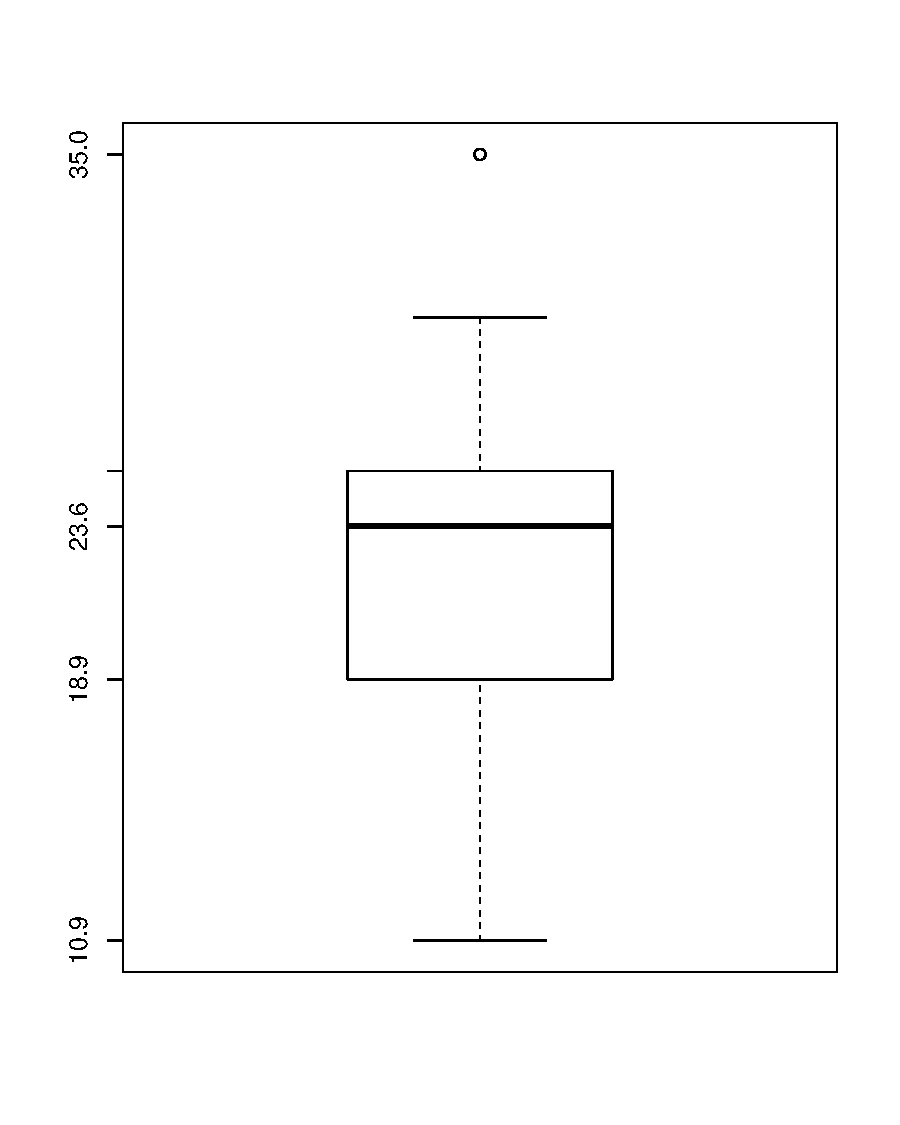
\includegraphics[width=0.9\linewidth]{exercicios-encontro2-solucao_files/figure-beamer/unnamed-chunk-5-1} \end{center}

\endColumns
\end{frame}

\begin{frame}{Exercício 1}
\phantomsection\label{exercuxedcio-1-3}
\small

\begin{longtable}[]{@{}
  >{\raggedleft\arraybackslash}p{(\linewidth - 10\tabcolsep) * \real{0.0429}}
  >{\raggedleft\arraybackslash}p{(\linewidth - 10\tabcolsep) * \real{0.0714}}
  >{\raggedleft\arraybackslash}p{(\linewidth - 10\tabcolsep) * \real{0.2429}}
  >{\raggedleft\arraybackslash}p{(\linewidth - 10\tabcolsep) * \real{0.2714}}
  >{\raggedleft\arraybackslash}p{(\linewidth - 10\tabcolsep) * \real{0.2429}}
  >{\raggedleft\arraybackslash}p{(\linewidth - 10\tabcolsep) * \real{0.1286}}@{}}
\toprule\noalign{}
\begin{minipage}[b]{\linewidth}\raggedleft
i
\end{minipage} & \begin{minipage}[b]{\linewidth}\raggedleft
IMC
\end{minipage} & \begin{minipage}[b]{\linewidth}\raggedleft
Desv. abs. média
\end{minipage} & \begin{minipage}[b]{\linewidth}\raggedleft
Desv. abs. mediana
\end{minipage} & \begin{minipage}[b]{\linewidth}\raggedleft
Desv. quadrático
\end{minipage} & \begin{minipage}[b]{\linewidth}\raggedleft
z-escore
\end{minipage} \\
\midrule\noalign{}
\endhead
1 & 10.9 & 12.09 & 12.7 & 146.25 & -0.6919 \\
2 & 17.8 & 5.19 & 5.8 & 26.97 & -0.0158 \\
3 & 17.9 & 5.09 & 5.7 & 25.94 & -0.8779 \\
4 & 18.9 & 4.09 & 4.7 & 16.76 & 1.1844 \\
5 & 18.9 & 4.09 & 4.7 & 16.76 & 0.1026 \\
6 & 20.5 & 2.49 & 3.1 & 6.22 & -0.8610 \\
7 & 22.9 & 0.09 & 0.7 & 0.01 & 0.2378 \\
8 & 23.6 & 0.61 & 0.0 & 0.37 & 0.4575 \\
9 & 23.9 & 0.91 & 0.3 & 0.82 & 0.3223 \\
10 & 24.4 & 1.41 & 0.8 & 1.98 & -0.4215 \\
11 & 24.9 & 1.91 & 1.3 & 3.64 & 1.1168 \\
12 & 25.7 & 2.71 & 2.1 & 7.33 & 0.1533 \\
13 & 29.6 & 6.61 & 6.0 & 43.65 & -0.6919 \\
14 & 30.0 & 7.01 & 6.4 & 49.09 & -2.0443 \\
15 & 35.0 & 12.01 & 11.4 & 144.16 & 2.0296 \\
\bottomrule\noalign{}
\end{longtable}
\end{frame}

\begin{frame}{Exercício 1}
\phantomsection\label{exercuxedcio-1-4}
\begin{longtable}[]{@{}lr@{}}
\toprule\noalign{}
\endhead
Amplitude & 24.10 \\
Desvio absoluto médio (média) & 4.42 \\
Desvio absoluto médio (mediana) & 4.38 \\
Variância & 34.99 \\
Desvio padrão & 5.92 \\
Coeficiente de variação & 25.73 \\
\bottomrule\noalign{}
\end{longtable}
\end{frame}

\section{Exercício 2}\label{exercuxedcio-2}

\begin{frame}{Exercício 2}
\phantomsection\label{exercuxedcio-2-1}
Uma pesquisa tinha como objetivo verificar qual o meio de transporte
mais comum entre os alunos de uma turma. As respostas foram:

\begin{longtable}[]{@{}
  >{\raggedright\arraybackslash}p{(\linewidth - 20\tabcolsep) * \real{0.0411}}
  >{\raggedright\arraybackslash}p{(\linewidth - 20\tabcolsep) * \real{0.0822}}
  >{\raggedright\arraybackslash}p{(\linewidth - 20\tabcolsep) * \real{0.0959}}
  >{\raggedright\arraybackslash}p{(\linewidth - 20\tabcolsep) * \real{0.0959}}
  >{\raggedright\arraybackslash}p{(\linewidth - 20\tabcolsep) * \real{0.0959}}
  >{\raggedright\arraybackslash}p{(\linewidth - 20\tabcolsep) * \real{0.0822}}
  >{\raggedright\arraybackslash}p{(\linewidth - 20\tabcolsep) * \real{0.0959}}
  >{\raggedright\arraybackslash}p{(\linewidth - 20\tabcolsep) * \real{0.0822}}
  >{\raggedright\arraybackslash}p{(\linewidth - 20\tabcolsep) * \real{0.1370}}
  >{\raggedright\arraybackslash}p{(\linewidth - 20\tabcolsep) * \real{0.0959}}
  >{\raggedright\arraybackslash}p{(\linewidth - 20\tabcolsep) * \real{0.0959}}@{}}
\toprule\noalign{}
\endhead
& Carro & Ônibus & Ônibus & Outro & Carro & A pé & Outro & Moto & Moto &
Carro \\
& Carro & Carro & Moto & Ônibus & Moto & Ônibus & Moto & Bicicleta &
Ônibus & Moto \\
& Outro & Carro & Moto & Carro & Carro & Ônibus & Carro & Ônibus & A pé
& Ônibus \\
\bottomrule\noalign{}
\end{longtable}

Obtenha uma medida de variabilidade adequada.
\end{frame}

\begin{frame}{Exercício 2}
\phantomsection\label{exercuxedcio-2-2}
\beginAHalfColumn

\begin{longtable}[]{@{}lrr@{}}
\toprule\noalign{}
Respostas & \(f_a\) & \(f_r\) \\
\midrule\noalign{}
\endhead
Carro & 9 & 0.300 \\
Ônibus & 8 & 0.267 \\
Moto & 7 & 0.233 \\
Outro & 3 & 0.100 \\
A pé & 2 & 0.067 \\
Bicicleta & 1 & 0.033 \\
Total & 29 & 0.967 \\
\bottomrule\noalign{}
\end{longtable}

\endColumns
\beginAHalfColumn

\begin{center}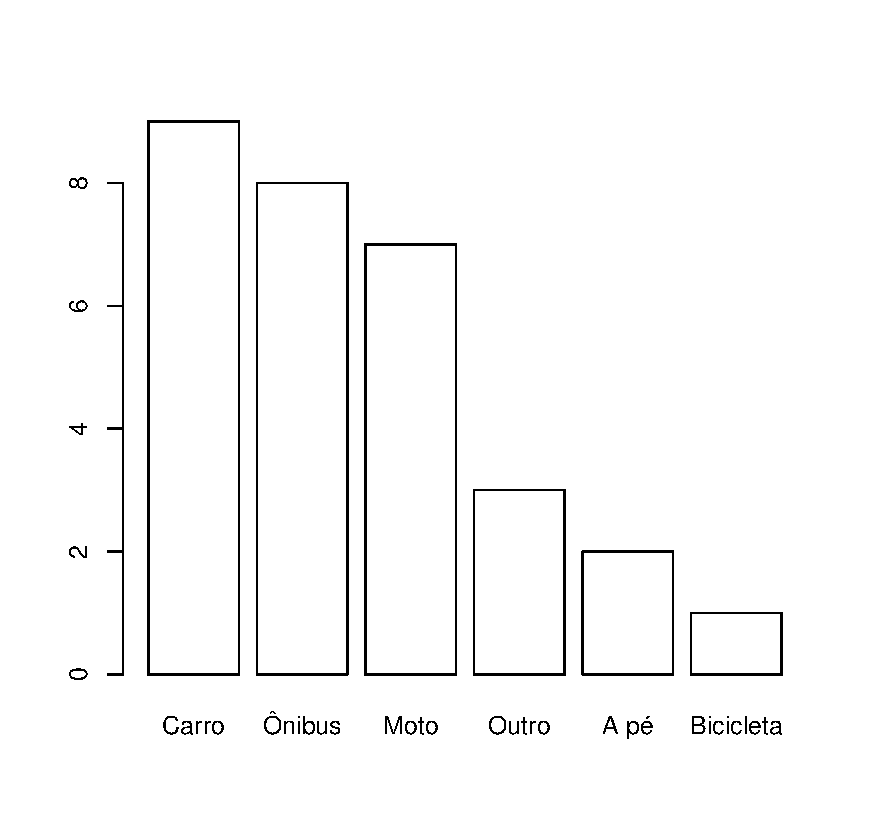
\includegraphics[width=0.9\linewidth]{exercicios-encontro2-solucao_files/figure-beamer/unnamed-chunk-10-1} \end{center}

\endColumns
\end{frame}

\begin{frame}{Exercício 2}
\phantomsection\label{exercuxedcio-2-3}
\beginAHalfColumn

\begin{longtable}[]{@{}lrr@{}}
\toprule\noalign{}
Respostas & \(f_a\) & \(f_r\) \\
\midrule\noalign{}
\endhead
Carro & 9 & 0.300 \\
Ônibus & 8 & 0.267 \\
Moto & 7 & 0.233 \\
Outro & 3 & 0.100 \\
A pé & 2 & 0.067 \\
Bicicleta & 1 & 0.033 \\
Total & 29 & 0.967 \\
\bottomrule\noalign{}
\end{longtable}

\begin{longtable}[]{@{}lr@{}}
\toprule\noalign{}
\endhead
H = & 1.58 \\
\bottomrule\noalign{}
\end{longtable}

\endColumns
\beginAHalfColumn

\begin{center}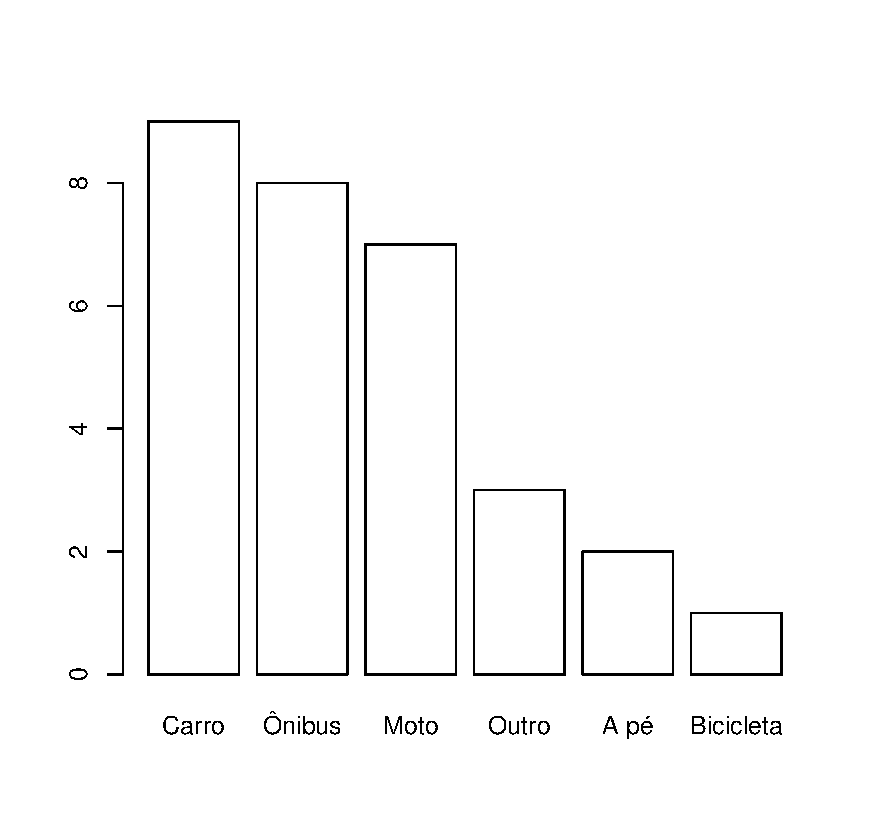
\includegraphics[width=0.9\linewidth]{exercicios-encontro2-solucao_files/figure-beamer/unnamed-chunk-13-1} \end{center}

\endColumns
\end{frame}

\section{Exercício 3}\label{exercuxedcio-3}

\begin{frame}{Exercício 3}
\phantomsection\label{exercuxedcio-3-1}
Em um estudo, uma universidade selecionou uma amostra de 10 alunos
pertencentes a 2 turmas. Destes alunos, registrou-se se tinha ou não
feito um curso pré vestibular e qual a nota obtida nas provas de
português e matemática. Os dados coletados estão na tabela abaixo.

\begin{longtable}[]{@{}rllrr@{}}
\toprule\noalign{}
Aluno & Turma & Curso & Português & Matemática \\
\midrule\noalign{}
\endhead
1 & A & Não & 4 & 4 \\
2 & B & Não & 3 & 3 \\
3 & B & Sim & 4 & 5 \\
4 & A & Não & 7 & 1 \\
5 & B & Não & 6 & 5 \\
6 & B & Não & 5 & 4 \\
7 & B & Não & 3 & 9 \\
8 & A & Sim & 4 & 9 \\
9 & A & Não & 10 & 6 \\
10 & B & Sim & 7 & 3 \\
\bottomrule\noalign{}
\end{longtable}
\end{frame}

\begin{frame}{Exercício 3}
\phantomsection\label{exercuxedcio-3-2}
\begin{enumerate}
\item
  Para turma e curso, obtenha tabelas de dupla entrada usando frequência
  absoluta e relativa (total, por linha e por coluna) e esboce gráficos
  adequados para representar as tabelas.
\item
  Obtenha uma medida de associação para turma e curso.
\item
  Para as notas, obtenha o coeficiente de correlação de Pearson e o
  diagrama de dispersão.
\item
  Obtenha medidas descritivas e box-plots das notas em função do curso e
  da turma.
\end{enumerate}
\end{frame}

\begin{frame}{1 Tabela de dupla entrada com frequências absolutas}
\phantomsection\label{tabela-de-dupla-entrada-com-frequuxeancias-absolutas}
\beginAThirdColumn

\begin{longtable}[]{@{}lrr@{}}
\toprule\noalign{}
& Não & Sim \\
\midrule\noalign{}
\endhead
A & 3 & 1 \\
B & 4 & 2 \\
\bottomrule\noalign{}
\end{longtable}

\endColumns
\beginTwoThirdsColumn

\begin{center}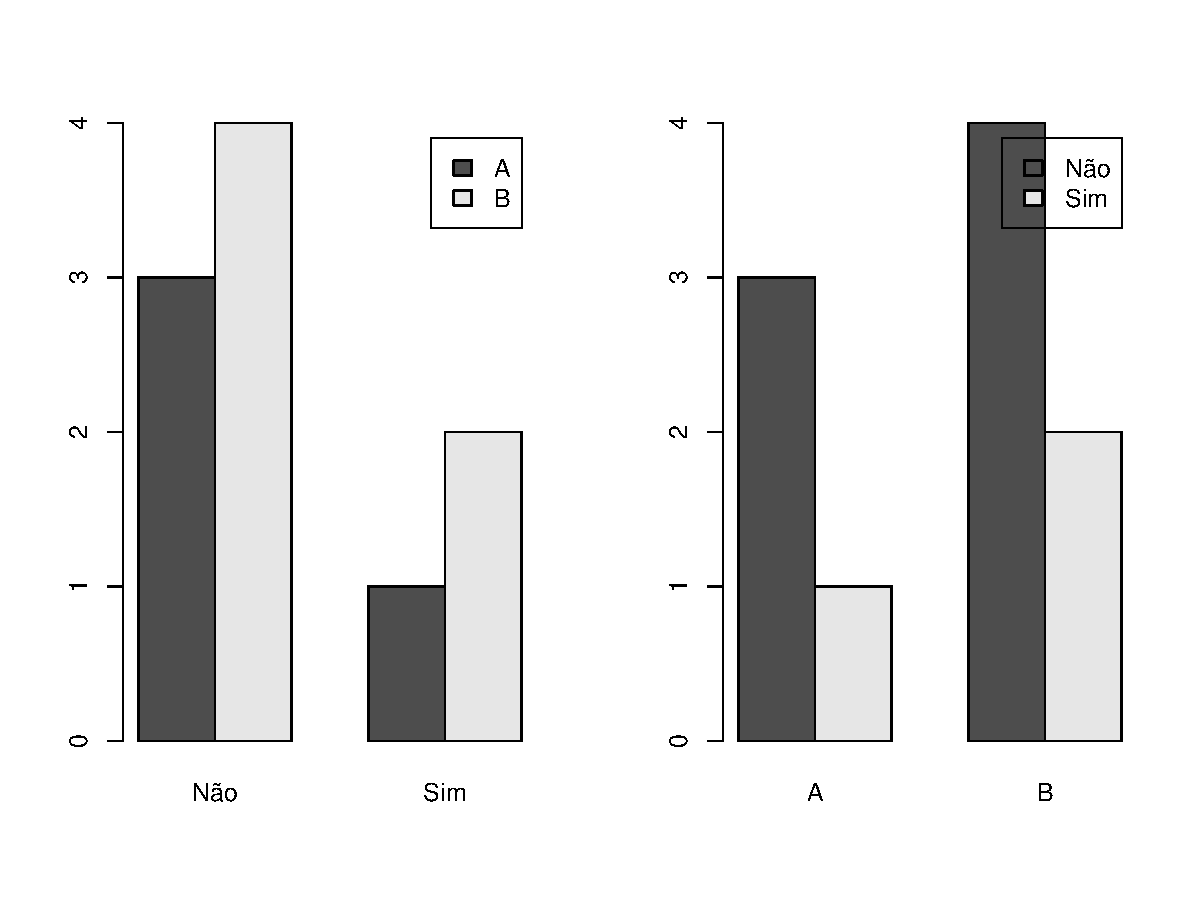
\includegraphics[width=11cm]{exercicios-encontro2-solucao_files/figure-beamer/unnamed-chunk-16-1} \end{center}

\endColumns
\end{frame}

\begin{frame}{1 Tabela de dupla entrada com frequências relativas (total
geral)}
\phantomsection\label{tabela-de-dupla-entrada-com-frequuxeancias-relativas-total-geral}
\beginAThirdColumn

\begin{longtable}[]{@{}lrr@{}}
\toprule\noalign{}
& Não & Sim \\
\midrule\noalign{}
\endhead
A & 0.3 & 0.1 \\
B & 0.4 & 0.2 \\
\bottomrule\noalign{}
\end{longtable}

\endColumns
\beginTwoThirdsColumn

\begin{center}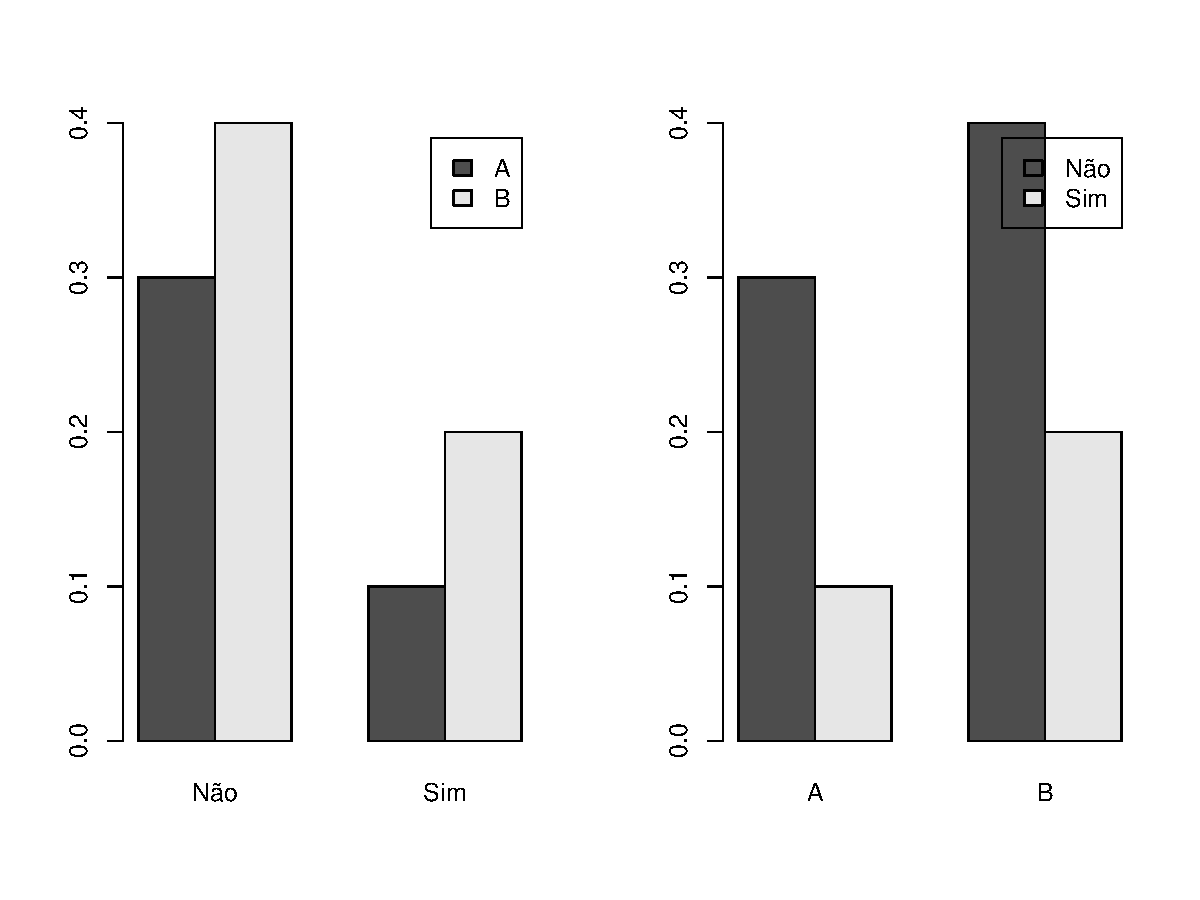
\includegraphics[width=11cm]{exercicios-encontro2-solucao_files/figure-beamer/unnamed-chunk-18-1} \end{center}

\endColumns
\end{frame}

\begin{frame}{1 Tabela de dupla entrada com frequências relativas (total
linha)}
\phantomsection\label{tabela-de-dupla-entrada-com-frequuxeancias-relativas-total-linha}
\beginAThirdColumn

\begin{longtable}[]{@{}lrrr@{}}
\toprule\noalign{}
& Não & Sim & Sum \\
\midrule\noalign{}
\endhead
A & 0.75 & 0.25 & 1 \\
B & 0.67 & 0.33 & 1 \\
Sum & 1.42 & 0.58 & 2 \\
\bottomrule\noalign{}
\end{longtable}

\endColumns
\beginTwoThirdsColumn

\begin{center}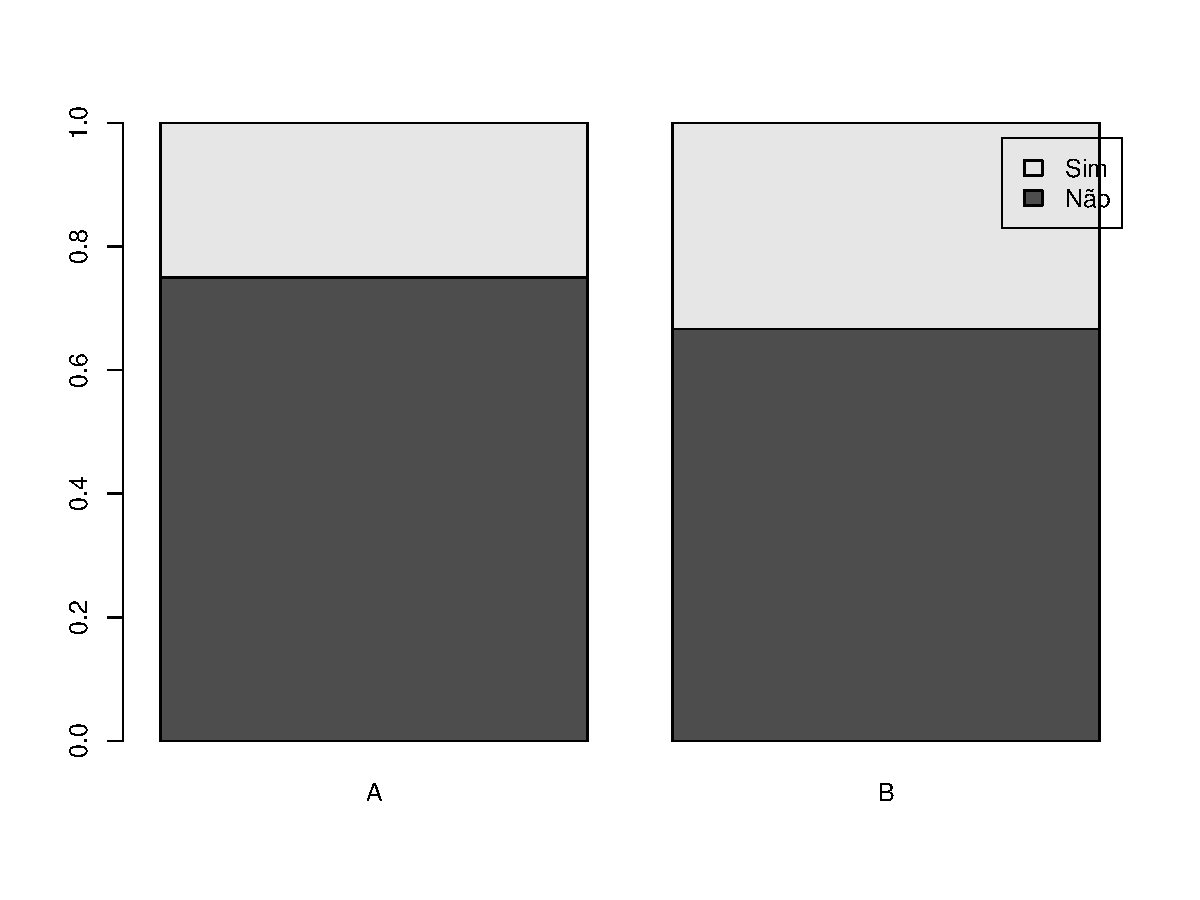
\includegraphics[width=11cm]{exercicios-encontro2-solucao_files/figure-beamer/unnamed-chunk-20-1} \end{center}

\endColumns
\end{frame}

\begin{frame}{1 Tabela de dupla entrada com frequências relativas (total
coluna)}
\phantomsection\label{tabela-de-dupla-entrada-com-frequuxeancias-relativas-total-coluna}
\beginAThirdColumn

\begin{longtable}[]{@{}lrrr@{}}
\toprule\noalign{}
& Não & Sim & Sum \\
\midrule\noalign{}
\endhead
A & 0.43 & 0.33 & 0.76 \\
B & 0.57 & 0.67 & 1.24 \\
Sum & 1.00 & 1.00 & 2.00 \\
\bottomrule\noalign{}
\end{longtable}

\endColumns
\beginTwoThirdsColumn

\begin{center}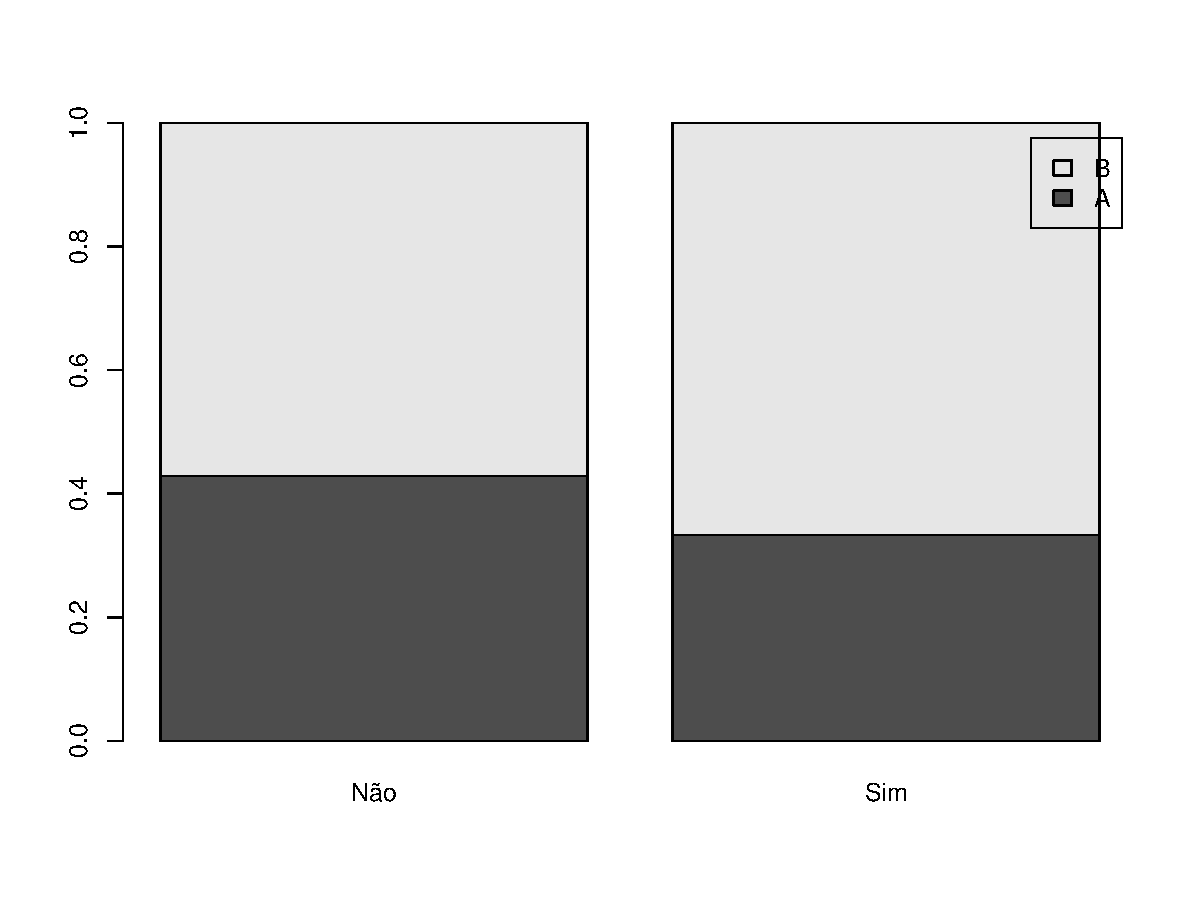
\includegraphics[width=11cm]{exercicios-encontro2-solucao_files/figure-beamer/unnamed-chunk-22-1} \end{center}

\endColumns
\end{frame}

\begin{frame}{2 Qui-quadrado para associação}
\phantomsection\label{qui-quadrado-para-associauxe7uxe3o}
\beginAHalfColumn

\begin{longtable}[]{@{}lccc@{}}
\caption{Valores observados.}\tabularnewline
\toprule\noalign{}
& Não & Sim & Total \\
\midrule\noalign{}
\endfirsthead
\toprule\noalign{}
& Não & Sim & Total \\
\midrule\noalign{}
\endhead
A & 3 & 1 & 4 \\
B & 4 & 2 & 6 \\
Total & 7 & 3 & 10 \\
\bottomrule\noalign{}
\end{longtable}

\begin{longtable}[]{@{}lccc@{}}
\caption{Valores esperados.}\tabularnewline
\toprule\noalign{}
& Não & Sim & Total \\
\midrule\noalign{}
\endfirsthead
\toprule\noalign{}
& Não & Sim & Total \\
\midrule\noalign{}
\endhead
A & 2.8 & 1.2 & 4 \\
B & 4.2 & 1.8 & 6 \\
Total & 7.0 & 3.0 & 10 \\
\bottomrule\noalign{}
\end{longtable}

\endColumns
\beginAHalfColumn

\begin{longtable}[]{@{}lcc@{}}
\caption{\(\frac{(o-e)^2}{e}\).}\tabularnewline
\toprule\noalign{}
& Não & Sim \\
\midrule\noalign{}
\endfirsthead
\toprule\noalign{}
& Não & Sim \\
\midrule\noalign{}
\endhead
A & 0.01 & 0.03 \\
B & 0.01 & 0.02 \\
\bottomrule\noalign{}
\end{longtable}

\[Q = \sum_{i=1}^{r} \sum_{j=1}^{s} \frac{(o_{ij} - e_{ij})^2}{e_{ij}} \approx  0\]
\endColumns
\end{frame}

\begin{frame}{3 Correlação}
\phantomsection\label{correlauxe7uxe3o}
\footnotesize

\begin{longtable}[]{@{}
  >{\centering\arraybackslash}p{(\linewidth - 12\tabcolsep) * \real{0.0256}}
  >{\centering\arraybackslash}p{(\linewidth - 12\tabcolsep) * \real{0.1410}}
  >{\centering\arraybackslash}p{(\linewidth - 12\tabcolsep) * \real{0.1667}}
  >{\centering\arraybackslash}p{(\linewidth - 12\tabcolsep) * \real{0.0256}}
  >{\centering\arraybackslash}p{(\linewidth - 12\tabcolsep) * \real{0.1410}}
  >{\centering\arraybackslash}p{(\linewidth - 12\tabcolsep) * \real{0.1667}}
  >{\centering\arraybackslash}p{(\linewidth - 12\tabcolsep) * \real{0.3333}}@{}}
\toprule\noalign{}
\begin{minipage}[b]{\linewidth}\centering
PT
\end{minipage} & \begin{minipage}[b]{\linewidth}\centering
\(PT - \overline{PT}\)
\end{minipage} & \begin{minipage}[b]{\linewidth}\centering
\((PT - \overline{PT})^2\)
\end{minipage} & \begin{minipage}[b]{\linewidth}\centering
MT
\end{minipage} & \begin{minipage}[b]{\linewidth}\centering
\(MT - \overline{MT}\)
\end{minipage} & \begin{minipage}[b]{\linewidth}\centering
\((MT - \overline{MT})^2\)
\end{minipage} & \begin{minipage}[b]{\linewidth}\centering
\((PT - \overline{PT}) \times (MT - \overline{MT})\)
\end{minipage} \\
\midrule\noalign{}
\endhead
4 & -1.3 & 1.69 & 4 & -0.9 & 0.81 & 1.17 \\
3 & -2.3 & 5.29 & 3 & -1.9 & 3.61 & 4.37 \\
4 & -1.3 & 1.69 & 5 & 0.1 & 0.01 & -0.13 \\
7 & 1.7 & 2.89 & 1 & -3.9 & 15.21 & -6.63 \\
6 & 0.7 & 0.49 & 5 & 0.1 & 0.01 & 0.07 \\
5 & -0.3 & 0.09 & 4 & -0.9 & 0.81 & 0.27 \\
3 & -2.3 & 5.29 & 9 & 4.1 & 16.81 & -9.43 \\
4 & -1.3 & 1.69 & 9 & 4.1 & 16.81 & -5.33 \\
10 & 4.7 & 22.09 & 6 & 1.1 & 1.21 & 5.17 \\
7 & 1.7 & 2.89 & 3 & -1.9 & 3.61 & -3.23 \\
\bottomrule\noalign{}
\end{longtable}

\footnotesize

\begin{longtable}[]{@{}lc@{}}
\toprule\noalign{}
\endhead
\(\overline{PT} =\) & 5.30 \\
\(\overline{MT} =\) & 4.90 \\
\(V(PT) =\) & 4.90 \\
\(V(MT) =\) & 6.54 \\
\(COV(PT,MT) =\) & -1.52 \\
\(COR(PT,MT) =\) & -0.27 \\
\bottomrule\noalign{}
\end{longtable}
\end{frame}

\begin{frame}{3 Diagrama de dispersão}
\phantomsection\label{diagrama-de-dispersuxe3o}
\begin{center}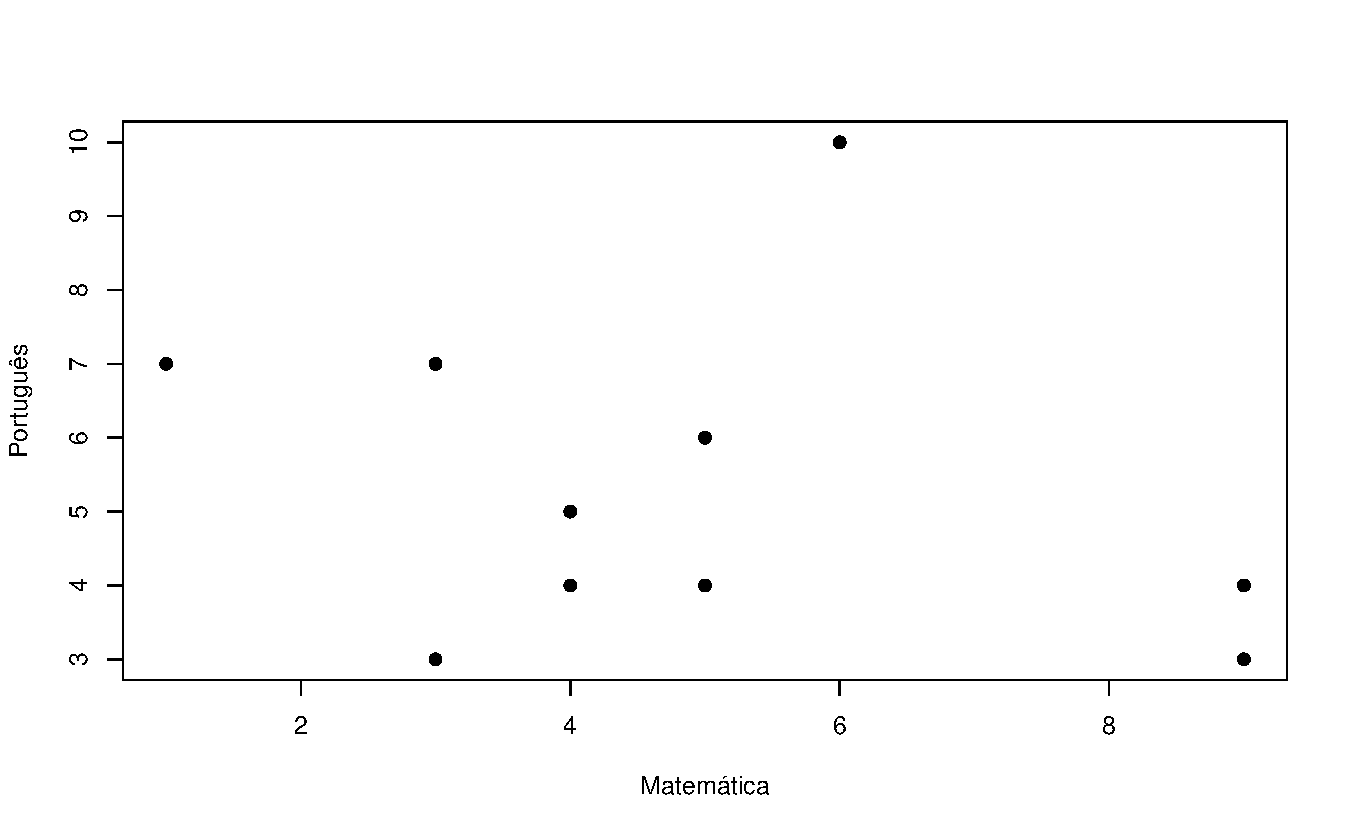
\includegraphics[width=11cm]{exercicios-encontro2-solucao_files/figure-beamer/unnamed-chunk-27-1} \end{center}
\end{frame}

\begin{frame}{4 Medidas descritivas por turma e curso}
\phantomsection\label{medidas-descritivas-por-turma-e-curso}
\beginAHalfColumn

\small

\begin{longtable}[]{@{}cccc@{}}
\caption{Notas em português em função do turma.}\tabularnewline
\toprule\noalign{}
Turma & Média & Mediana & Desvio padrão \\
\midrule\noalign{}
\endfirsthead
\toprule\noalign{}
Turma & Média & Mediana & Desvio padrão \\
\midrule\noalign{}
\endhead
A & 6.25 & 5.5 & 2.87 \\
B & 4.67 & 4.5 & 1.63 \\
\bottomrule\noalign{}
\end{longtable}

\begin{longtable}[]{@{}cccc@{}}
\caption{Notas em matemática em função do turma.}\tabularnewline
\toprule\noalign{}
Turma & Média & Mediana & Desvio padrão \\
\midrule\noalign{}
\endfirsthead
\toprule\noalign{}
Turma & Média & Mediana & Desvio padrão \\
\midrule\noalign{}
\endhead
A & 5.00 & 5.0 & 3.37 \\
B & 4.83 & 4.5 & 2.23 \\
\bottomrule\noalign{}
\end{longtable}

\endColumns
\beginAHalfColumn

\small

\begin{longtable}[]{@{}cccc@{}}
\caption{Notas em português em função do curso.}\tabularnewline
\toprule\noalign{}
Curso & Média & Mediana & Desvio padrão \\
\midrule\noalign{}
\endfirsthead
\toprule\noalign{}
Curso & Média & Mediana & Desvio padrão \\
\midrule\noalign{}
\endhead
Não & 5.43 & 5 & 2.51 \\
Sim & 5.00 & 4 & 1.73 \\
\bottomrule\noalign{}
\end{longtable}

\begin{longtable}[]{@{}cccc@{}}
\caption{Notas em matemática em função do curso.}\tabularnewline
\toprule\noalign{}
Curso & Média & Mediana & Desvio padrão \\
\midrule\noalign{}
\endfirsthead
\toprule\noalign{}
Curso & Média & Mediana & Desvio padrão \\
\midrule\noalign{}
\endhead
Não & 4.57 & 4 & 2.51 \\
Sim & 5.67 & 5 & 3.06 \\
\bottomrule\noalign{}
\end{longtable}

\endColumns
\end{frame}

\begin{frame}{4 box-plots das notas em função de turma e curso}
\phantomsection\label{box-plots-das-notas-em-funuxe7uxe3o-de-turma-e-curso}
\begin{center}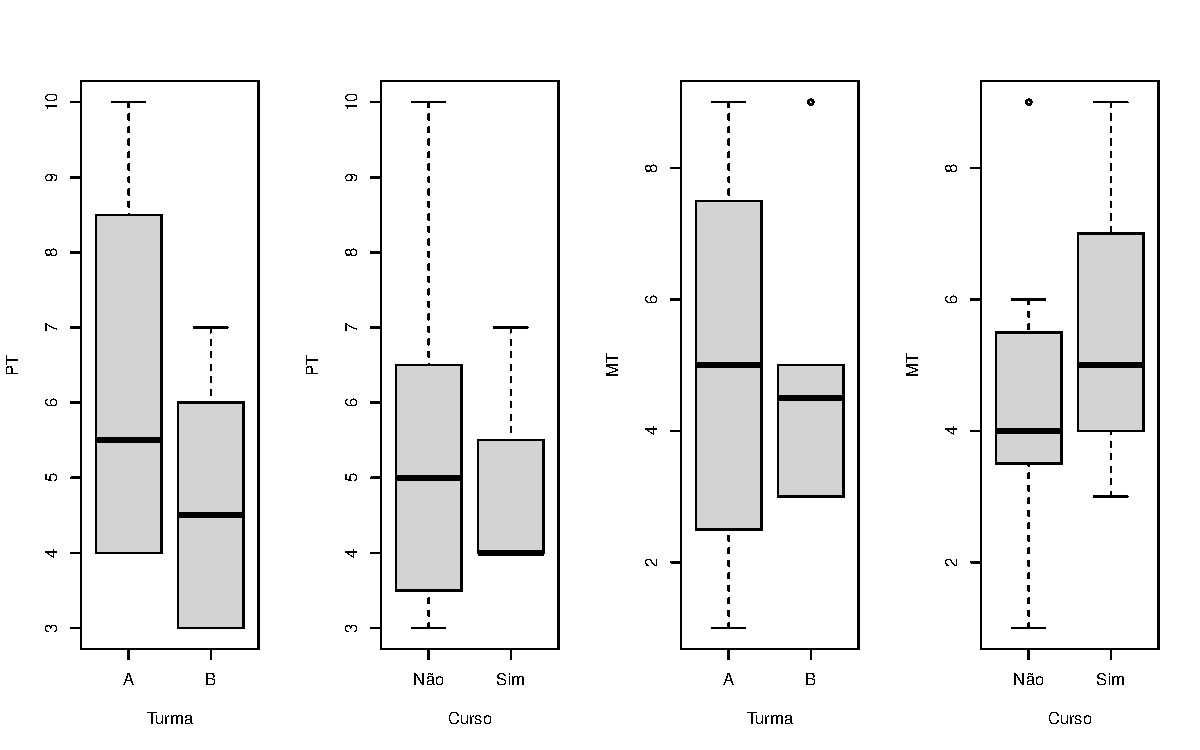
\includegraphics[width=11cm]{exercicios-encontro2-solucao_files/figure-beamer/unnamed-chunk-30-1} \end{center}
\end{frame}

\end{document}
